\documentclass[a4paper,11pt]{article}

\usepackage[frenchb]{babel}
\usepackage[utf8]{inputenc}
\usepackage{geometry}
\usepackage{listings}
\usepackage{multicol}
\usepackage{graphicx}
\usepackage[T1]{fontenc}

\usepackage{caption}
\DeclareCaptionFormat{legend}{#3}
\captionsetup{format=legend, font=small}

\geometry{hmargin=3cm,vmargin=4cm}

\newcommand{\CC}{C\nolinebreak\hspace{-.05em}\raisebox{.4ex}{\tiny\bf +}\nolinebreak\hspace{-.10em}\raisebox{.4ex}{\tiny\bf +}}

\newenvironment{custommargins}[2]{
     \addtolength{\leftskip}{#1}
     \addtolength{\rightskip}{#2}}{\par}



\begin{document}

\begin{titlepage}
\hspace{3cm}
\vspace{4cm}
\begin{center}
\begin{Huge}
\bfseries Application informatique
\end{Huge}
\vspace{3cm}

\begin{Huge}
\bfseries Another Side-scrolling Platformer Engine
\end{Huge}
\end{center}

\vspace{2cm}

\begin{center}
\begin{large}
\begin{tabular}{ll}
  Réalisé par~: & Séverine \textsc{Delaplace}\\
  				& Amaury \textsc{Fauvel}\\
                & Quentin \textsc{Godart}\\
                & Aurélien \textsc{Villette}\\
\end{tabular}
\end{large}
\end{center}
\end{titlepage}



%Table of contents
\newpage
\tableofcontents
\newpage

%Contents



\vspace{1cm}
\section{Introduction}
\subsection{Présentation}
Another Side-scrolling Platformer Engine (ASPE) est la démonstration d'un jeu-vidéo en 2 dimensions à défilement horizontal (la caméra se déplace latéralement avec le joueur). Le joueur s'y déplace librement avec les flèches du clavier et la barre d'espace.

Ce type de jeu figure parmi les plus représenté dans l'histoire du média interactif, avec de nombreux titres marquant comme Super Mario, Sonic the Hedgehog ou Rayman. Le but d'un tel jeu est de parcourir des niveaux (souvent de gauche à droite) parsemés d'obstacle et ennemis.

\vspace{0.6cm}
\begin{figure}[h]
\begin{center}
\includegraphics[scale=0.4]{mario.jpg}
\caption{Super Mario Bros - Ninendo - 1985}
\end{center}
\end{figure}

L'éxécutable se trouve dans \texttt{build-debug} sous le nom \texttt{./jeu2d}.

\subsection{Objectifs du projet}
Le but du projet est de réaliser un moteur graphique adapté aux jeux de plateforme. Il doit être doté d'une architecture robuste et extensible qui pourrait être utilisée dans le cadre d'un jeu complet. Le nombre de fonctionnalités est minimal car l'objectif est de fournir la base d'un jeu, et non un jeu complet.
    
\section{Choix de programmation et workflow}
\subsubsection*{Langage}
Le langage utilisé pour l'intégralité du projet est le \CC .
Le \CC est un langage orienté objet influencé par le C. Un de ses principaux atouts est la gestion fine des ressources et ses performances. C'est un langage de choix pour toute application en temps réel employant des calculs graphiqueset est couramment utilisé par les studios de développement de jeux.
C'est un langage que nous n'avons pas appris au cours de notre scolarité, c'était donc l'occasion pour nous de nous familiariser avec un nouveau langage.

\subsubsection*{Bibliothèque graphique}
La bibliothèque graphique employée est le Simple and Fast Multimedia Library (SFML). C'est une bibliothèque assez bas niveau, elle nous permet de gérer efficacement les ressources (images affichées). Elle a l'avantage d'être conçue pour les langages orientés objet, c'est pourquoi nous l'avons préféré à la Simple DirectMedia Layer (SDL).

La SFMl est séparée en différents modules :
\begin{itemize}
\item Window : gère l'ouverture de la fenêtre basée sur OpenGL. C'est dans ce contexte que se déroule le jeu. Sert aussi à récupérer les inputs du clavier.
\item Graphics : implémente le chargement de textures, l'affichage de sprites et la gestion de la caméra.
\item System : pour les configurations diveres (taux de rafraîchissement notamment)
\item Sound : gère les sons et pistes audio (malheureusement non utilisé ici)
\item Network : pour les communications en réseau (non utilisé ici)
\end{itemize}

\subsubsection*{Méthodes de travail}
Nous avons choisi l'environnement de développement CLion (de la suite JetBrains) pour ses fonctionnalités utiles comme l'intégration de Git, notre gestionnaire de versions.

Comme outil de communication, nous avons utilisé Slack. Slack est une application web de chat adapté au monde du travail grâce à son système de salon et à la centralisation d'autre application comme Trello.

Trello se présente sous la forme d'un tableau où l'on affiche les différentes tâches à faire, en cours et terminées, assignables aux membres du groupe.
Finalement, nous avons rarement utilisé Trello car nous n'étions que 4 et nous côtoyons tous les jours.

\section{Implémentation}
La qualité de l'architecture était notre principale préoccupation. Elle permet d'avoir une base de jeu largement extensible, car la quasi-totalité des fonctionnalités d'un jeu complet ne concernent que des ajouts au modèle du jeu.

Nous avons choisi une architecture Modèle-Vue-Contrôleur. Elle permet une grande maintenabilité et une clarté du code. De plus elle connaît son lot de bonne pratique qui assure la robustesse du programme.

Le jeu étant en temps réel, une boucle principale tourne jusqu'à la fermeture de la fenêtre. Dans cette boucle, la classe principale \texttt{Game} agit comme un chef d'orchestre et appelle tour à tour le \texttt{EventHandler} qui récupère les inputs clavier, le \texttt{GameModel} qui met à jour tout le modèle à partir des inputs récupérés, et le \texttt{GraphicRenderer} qui affiche le niveau et les entités qui y évoluent. Un tour de boucle est l'unité temporelle de base, appelé $tick$.

\begin{center}
\includegraphics[scale=0.6]{architecture.jpg}
\end{center}





Ces trois gestionnaires ne devraient être instancié qu'une seule fois. Nous avons pensé à les implémenter suivant le patron de conception singleton mais cela compliquait un code qui n'a pas pour but d'être distribué et utilisé largement (dans une équipe réduite aucun de nous n'aurait essayé de créer plusieurs de ces objets).

\subsection{Contrôleur}
La partie contrôle est la plus simple : le \texttt{EventHandler}, par sa méthode \texttt{pullEvents()}, récupère l'état de chaque touches associée à un contrôle avec la méthode SFML :
\begin{multicols}{2}{
\begin{lstlisting}
     sf::KeyBoard::isKeyPressed()
\end{lstlisting}

L'association  entre les contrôles (directions, saut) et les touches du clavier (espace, flèches) est faite par l'espace de noms \texttt{Controls}.


\fbox{
\begin{minipage}{7cm}
	Note : en \CC , pour \texttt{Nom::fonction()},
    \texttt{Nom} est un espace de nom pour une
     collection de fonctions utilitaires.\\
     \texttt{sf} est l'espace de nom de la SFML.
\end{minipage}
}
\vspace{1cm}
}
\end{multicols}


\subsection{Modèle}
La classe \texttt{GameModel} s'occupe de modéliser le jeu. sa méthode principale, \texttt{update()}, fait se dérouler un tour de jeu et met à jour toutes ses composantes.

\subsubsection*{Level}
Le jeu étant en 2 dimensions, tous les objets évoluent sur un repère orthonormé dont l'unité est le pixel. l'origine du repère se situe en haut à gauche du niveau, les coordonnées dans le niveau sont donc positives ($x$ augmente en allant vers la droite et $y$ augmente en allant vers le bas).

Le terrain du niveau est décomposé en blocs de $16 \times 16$ pixels alignés sur une grille. Les blocs sont représentés par des entiers codés sur 1 octet. Ils sont énumérés dans l'espace de nom \texttt{Blocks}.

Il existe 3 types fondamentaux de blocs : l' \texttt{Air} pour l'espace libre, le \texttt{Ground} pour le sol et le \texttt{Wall} pour les murs et plafond. On ne testera les collisions que vers le bas dans le cas d'un \texttt{Ground}, ce qui limite le nombre d'opérations. (voir Collisions) alors que le \texttt{Wall} est solide dans toutes les directions.

Ces deux derniers blocs sont déclinés en 3 types de pentes ($45^\circ$, $22,5^\circ$ et $67,5^\circ$) déclinées dans toutes les directions.

\begin{center}
\includegraphics[scale=0.6]{pente.jpg}
\end{center}

Cette variété de blocs entraîne la présence de 42 items, que la classe \texttt{Blocks} encapsule avec les fonctions suivantes :
\vspace{0.3cm}

\renewcommand{\arraystretch}{1.3}
\begin{tabular}{r | l}
\begin{lstlisting}
isGround(block b)
\end{lstlisting}
& Renvoie $VRAI$ si $b$ est un sol ou dérivés \\
\begin{lstlisting}
isWall(block b)
\end{lstlisting}
& Renvoie $VRAI$ si $b$ est un mur ou dérives \\
\begin{lstlisting}
isAir(block b)
\end{lstlisting}
& Renvoie $VRAI$ si $b$ est vide \\
\begin{lstlisting}
isSlope(block b)
\end{lstlisting}
& Renvoie $VRAI$ si $b$ est une pente \\
\begin{lstlisting}
isUp(block b)
\end{lstlisting}
& Renvoie $VRAI$ si $b$ est une pente montante \\
\begin{lstlisting}
isDown(block b)
\end{lstlisting}
& Renvoie $VRAI$ si $b$ est une pente de plafond \\
\begin{lstlisting}
slope(int x, block b)
\end{lstlisting}
& Renvoie la hauteur $y$ correspondant au \\
& décalage $x$ horizontal dans le bloc

\end{tabular}

\vspace{0.4cm}
Les terrains de niveaux sont stockés dans des fichiers à l'emplacement \texttt{asset/map/$niveau$/level.bin} dans une matrice d'entiers codant les blocs. Il est à noter que le terrain du niveau et son affichage sont séparés et indépendant (voir LevelView dans la partie Vue).

\begin{center}
\includegraphics[scale=0.5]{level.jpg}
\end{center}

\vspace{1cm}
Actuellement il n'est pas permis à l'utilisateur de changer de niveau. Seul le niveau de test est chargé au lancement.


\subsubsection*{Player}
La classe \texttt{Player} implémente l'entité que contrôle l'utilisateur. Ses principaux attributs sont sa position et sa vitesse (en $pixel/tick$) représentés par des couples d'entier (\texttt{Pair}). Chaque tour de jeu, le \texttt{GameModel} ajuste la vitesse du \texttt{Player} en fonction des inputs récupérés. Puis le \texttt{Player} se met à jour selon son comportement :
\begin{enumerate}
\item La gravité augmente la vitesse dans les positifs (vers le bas).
\item Le frottement réduit la vitesse horizontale. Ainsi la vitesse est réduite progressivement dans les sauts.
\item On empêche les vitesses de dépasser un maximum.
\item Si on est sur le sol et que la vitesse est positive (vers le bas), on ramène à 0 la vitesse.
\item On essaie de se déplacer de $speed$ pixels, en appliquant les collisions (voir \texttt{CollisionHandler}).
\end{enumerate}

Actuellement le \texttt{Player} est la seule entité du jeu. Pour un moteur de jeu plus complet il aurait fallu gérer un ensemble d'\texttt{Entity} et appliquer une fonction \texttt{update()} à chacune d'elle. L'affichage aurait aussi d'afficher les entités une à une.

\subsubsection*{CollisionHandler}
Le gestionnaire de collision est l'outil qui indique au \texttt{Player} les blocs avec lesquels il entrera en collision. Sa principale méthode est :
\begin{lstlisting}
        std::vector<block> getColliders(Pair pos, Pair size);
\end{lstlisting}

Cette méthode prends en paramètres deux couples d'entier : la position hypothétique et la taille de l'entité. Le \texttt{CollisionHandler} teste chaque pixel de la zone et ajoute chaque bloc trouvé dans un tableau dynamique (\texttt{vector} du \CC). La précision au pixel près est un peu plus coûteuse que de tester 1 pixel sur 16, mais cc'est le seul moyen de gérer les pentes.

Si le tableau renvoyé est vide, le joueur pourra se déplacer sans souci. Sinon il essaiera dans chaque direction de se déplacer pixel par pixel pour se coller au bloc sans rentrer dedans. Aussi il teste les pixels un peu au dessus pour monter la pente (et ne pas être bloqué par 1 pixel).

\vspace{1cm}
\begin{center}
\fbox{
\includegraphics[scale=0.6]{schema-collision.png}
}
\end{center}
\vspace{1cm}

\subsection{Vue}
C'est la partie la plus sensible car elle va déterminer les performances du moteur : les accès aux fichiers d'images, et le rendu graphique est ce qu'il y a de plus coûteux. C'est la classe \texttt{GraphicRenderer} qui fait la gestion des composantes graphiques. La méthode principale \texttt{render} prends en paramètre le \texttt{Player} du modèle, et s'occupe d'afficher son environnement.

\vspace{1cm}

\subsubsection*{sf\texttt{::}Sprite}
La SFML gère les images par des sprites. C'est à dire un rectangle d'une taille définie sur lequel est plaquée une texture. La texture est l'image du sprite. Lorsqu'on plaque une texture sur un sprite, on donne la partie de la texture que l'on veut garder.
Exemple :
\begin{center}
\begin{tabular}{|l}
\begin{lstlisting}
sf::Texture texture;
texture.loadFromFile("image.png");
sf::Sprite sprite;
sprite.setTexture(texture);
sprite.setTextureRect(sf::IntRect(10, 10, 32, 32);
\end{lstlisting}
\end{tabular}
\end{center}

Cette portion de code charge la texture stockée dans \texttt{image.png} et l'affecte à un sprite.
L'enjeu est de minimiser les appels à \texttt{loadFromFile()} et les déclarations de \texttt{sf::Texture}

\subsubsection*{LevelView}
La classe \texttt{LevelView} stocke la partie visuelle d'un niveau d'une manière similaire au \texttt{Level} du modèle : les tuiles (tiles) sont représentées par des entiers codés sur 1 octet et stocké dans un fichier binaire (emplacement \texttt{assets/map/$niveau$/view.bin}). Cette fois, pas d'énumération, car l'entier correspond directement au décalage de la tuile sur le tileset.


\begin{center}
\fbox{
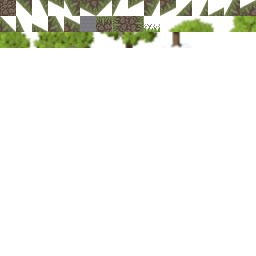
\includegraphics[scale=2]{tileset.png}
}
\end{center}

Ainsi, une seule image contient toutes les tuiles correspondant à une seule texture à plaquer sur un sprite. La différence visuelle entre deux sprites est uniquement due à la portion de texture plaquée avec \texttt{sprite.setTextureRect()}.

\subsubsection*{SpriteFactory}
Cette classe gère l'association d'un sprite à une entité. Pour cela le patron de conception fabrique a été employé : la méthode \texttt{sf::Sprite create(Player entity)} prends en paramètre une entité et renvoie le sprite adéquat. La feuille de sprite du joueur contient toutes les étapes de l'animation, et c'est la \texttt{SpriteFactory} qui affecte la bonne partie de l'animation en fonction de l'état du joueur.

Si le joueur est en l'air son sprite sera celui du saut/chute. Sinon un entier qui évolue de manière cyclique lorsque le joueur marche sert à choisir l'étape de l'animation de marche.

\vspace{0.7cm}
\begin{center}
\includegraphics[scale=0.5]{spritefactory.jpg}
\end{center}
\vspace{1cm}

\subsubsection*{sf::View}
La SFML gère la caméra par cette classe. Il suffit d'une translation de tout l'affichage vers une zone centrée sur le joueur pour avoir un défilement horizontal.
\begin{lstlisting}
camera.setCenter(player.pos.x, SCREEN_HEIGHT / 2);
\end{lstlisting}

\subsection{Éditeur de niveaux}
Nous avions prévu de créer un éditeur de niveau, mais étant un "accessoire" nous nous sommes concentrés sur le jeu. Pour créer un niveau, nous utilisons un éditeur de texte pour écrire les nombres en base 62 (chiffres, lettres minuscules et lettres majuscules). Un programme écrit en C fait la conversion vers un fichiers binaire avec les bons nombres.

\section{Répartition des tâches}
\begin{itemize}
\item[Amaury :] Base de l'architecture, gestion et affichage du niveau (\texttt{Level} et \texttt{LevelView}), outil de conversion texte - binaire.
\item[Aurélien :] Physique du joueur et collisions 
\item[Séverine :] Physique du joueur et collision, outils sur les blocs
\item[Quentin :] Association sprite-entité, dessin des sprites et création du niveau de démonstration.
\end{itemize}

    
\section{Pistes d'amélioration}
Pour graphique minimal mais complet, il aurait fallut gérer une liste d'entités et pas un unique \texttt{Player}.
\newline Aussi il faudrait un gestionnaire de niveaux pour pouvoir charger et décharger des environnements (pour recommencer un niveau à la mort, et passer au niveau suivant à la fin).
\newline Enfin, nous n'avons pas prévu l'affichage d'interface (informations sur le joueur, bulles de texte...)

\section{Conclusion}
En faisant le choix de développer ce projet en \CC avec la bibliothèque SFML nous nous sommes imposé une première difficulté, celle d'apprendre le langage et son fonctionnement avec la bibliothèque graphique.

De plus, l'idée du sujet étant notre initiative nous avons du nous même établir une ligne directrice et nous y tenir.
Le sujet étant vaste et nouveau, nous avons dû apprendre les différentes principes de fonctionnement de moteurs graphiques ceux qui nous a valu d'explorer de nombreuses pistes.

Ce projet nous a apporté de l'expérience sur un nouveau type d'application, sur un travail en groupe plus poussé pendant une durée plus longue, sur la gestion d'un projet en partant de sa création et sur l'apprentissage d'un nouveau langage avec de nouveaux outils.

\end{document}
